\documentclass[11pt, letterpaper]{article}
\setlength{\parindent}{0in}
\setlength{\textheight}{8.7in}
\setlength{\textwidth}{6.8in}
\setlength{\oddsidemargin}{-0.3in}
\setlength{\evensidemargin}{0.0in}
\addtolength{\topmargin}{-1in}
\setlength{\parskip}{0.1in}

\usepackage{amsmath, amsfonts, color}
\usepackage{bm}
\usepackage{enumerate}
\usepackage{graphicx}
\usepackage{pdflscape}
\usepackage{afterpage}
\usepackage{capt-of}
\newcommand*{\justifyheading}{\raggedleft}

\usepackage[top=1in, bottom=1.25in, left=1.25in, right=1.25in]{geometry}




\renewcommand{\baselinestretch}{1.0}

\newcommand{\bx}{{\bm x}}
\newcommand{\bX}{{\bm X}}
\newcommand{\by}{{\bm y}}
\newcommand{\bY}{{\bm Y}}
\newcommand{\bW}{{\bm W}}
\newcommand{\bG}{{\bm G}}
\newcommand{\bR}{{\bm R}}
\newcommand{\bZ}{{\bm Z}}
\newcommand{\bV}{{\bm V}}
\newcommand{\bL}{{\bm L}}
\newcommand{\bz}{{\bm z}}
\newcommand{\be}{{\bm e}}
\newcommand{\bgamma}{{\bm \gamma}}
\newcommand{\bbeta}{{\bm \beta}}
\newcommand{\balpha}{{\bm \alpha}}
\newcommand{\bSigma}{{\bm \Sigma}}
\newcommand{\bmu}{{\bm \mu}}
\newcommand{\btheta}{{\bm \theta}}
\newcommand{\bepsilon}{{\bm \epsilon}}
\newcommand{\bone}{{\bm 1}}
\newcommand{\bzero}{{\bm 0}}
\newcommand{\bC}{{\bm C}}
\newcommand{\bI}{{\bm I}}
\newcommand{\bA}{{\bm A}}
\newcommand{\bB}{{\bm B}}
\newcommand{\bQ}{{\bm Q}}
\newcommand{\bS}{{\bm S}}
\newcommand{\bD}{{\bm D}}
\newcommand{\cQ}{\mathcal{Q}}
\newcommand{\cU}{\mathcal{U}}
\newcommand{\cI}{\mathcal{I}}
\newcommand{\cL}{\mathcal{L}}

\newcommand{\beas}{\begin{eqnarray*}}
\newcommand{\eeas}{\end{eqnarray*}}

\newenvironment{equationarrayright}{
                          \begin{eqnarray*}
                          \begin{array}{rcll}
                         }{
                          \end{array}
                          \end{eqnarray*}
                         }
\newcommand{\bear}{\begin{equationarrayright}}
\newcommand{\eear}{\end{equationarrayright}}


\DeclareMathOperator*{\argmin}{arg\,min}

\begin{document}

\Large 
\begin{center}
\bf Ferry Curious about WSDOT Sailing Times \\
\bf Mike Logsdon and Zach Stednick
\end{center} 
\normalsize 


Although the majority of posts on this blog cover Metro, we wanted to shift the focus a bit to look at another transit method - ferries. It seems that the majority of the coverage of WSDOT ferries focuses on the fiscal side such as costs of ferry maintenance and replacement as well was critical examinations of ferry employee salaries.
We wanted to shift the conversation slightly and focus on the logistical aspect of the ferry system. Are the ferries generally on time? Can delays be predicted? Are certain routes or vessels unusually punctual or unusually late? 
To achieve this we filed a Public Records Request to gain access to this data. Here we present findings for on-time rates for calendar year 2014. For simplicity this report considers Puget Sound ferry routes.

\begin{figure}
\begin{center}
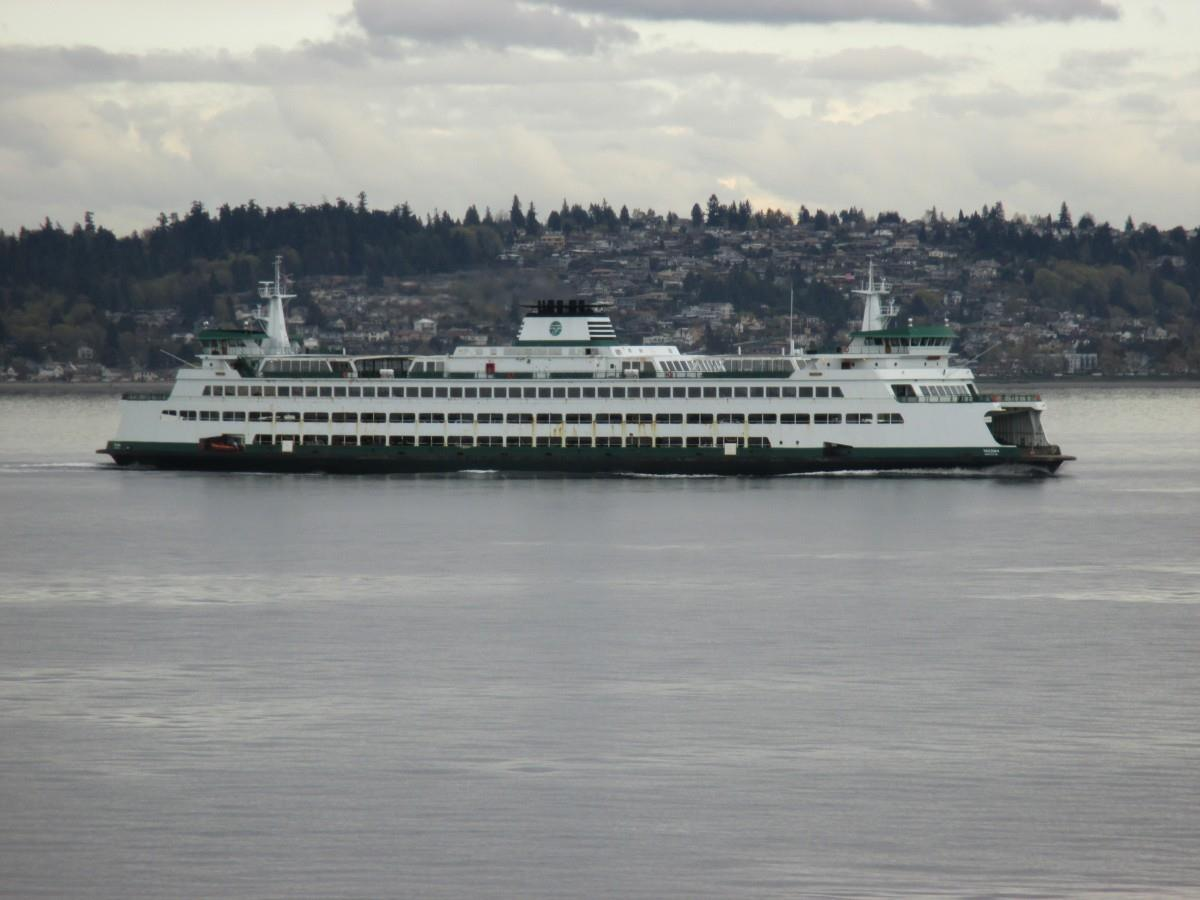
\includegraphics[scale = .4]{ferry.jpg}
\end{center}
\end{figure}

\section*{Summary}

High level findings, to fill in later. Summertime = trouble. Fauntleroy- Vashon-Southworth "Bermuda Triangle" = trouble. Point Defiance - Tahlequah is fantastic. System overall very reliable with a few weak points.


\section*{Departure Time - Actual versus Scheduled}

To investigate the reliability of the ferry system, we first examine actual departure time as compared to scheduled departure time. WSDOT uses GPS trackers to monitor each ferry and is therefore able to record arrival and departure times to the second. 

\subsection*{Data oddities}

As is the custom, daylight savings time tangles up the recording a few hours of the year. For example, a sailing from Seattle to Bainbridge island was scheduled for 2:10 AM on the morning of November 2, 2014, right at the end of daylight savings time. The actual departure time was recorded at 1:11 AM. This likely reflects the manner in which sailing times were reported during the daylight savings switch, rather than an instance of a boat leaving one hour ahead of schedule. For simplicity the small number of late night sailings at the margin of daylight savings time were excluded from the analysis.

In addition there were several records of boats leaving inexplicably early. The most extreme was a sailing from Vashon to Fauntleroy, scheduled for 8AM on the morning of April 26, 2014. The actual departure time was recorded at 1:21 AM, over six hours before the scheduled sailing.  These records were attributed as data entry errors and also excluded from analysis.


\subsection*{Routes and Vessels}


\afterpage{%
    \clearpage% Flush earlier floats (otherwise order might not be correct)
    \thispagestyle{empty}% empty page style (?)
    \begin{landscape}% Landscape page
        \centering % Center table
        \resizebox{24cm}{!} {
\begin{tabular}{ | r | p{2cm} | p{1.6cm} | p{1.8cm} | p{1.9cm} | p{1.8cm} | p{1.9cm} | p{1.7cm} | p{1.7cm} | p{1.7cm} | p{1cm} |}
  \hline
 & Fauntleroy- Southworth & Keystone- Port Townsend & Seattle- Bremerton & Southworth- Vashon & Point Defiance- Tahlequah & Seattle- Bainbridge & Edmonds- Kingston & Fauntleroy- Vashon & Mukilteo- Clinton & Total \\ 
  \hline
Yakima & 0 & 0 & 0 & 0 & 0 & 0 & 22 & 0 & 0 & 22 \\ 
  Hyak & 0 & 0 & 824 & 0 & 0 & 0 & 0 & 0 & 0 & 824 \\ 
  Chelan & 85 & 0 & 424 & 208 & 0 & 0 & 4 & 381 & 1032 & 2134 \\ 
  Kaleetan & 0 & 0 & 2645 & 0 & 0 & 0 & 0 & 0 & 0 & 2645 \\ 
  Kennewick & 0 & 3842 & 0 & 0 & 0 & 0 & 0 & 0 & 0 & 3842 \\ 
  Evergreen & 494 & 0 & 0 & 1387 & 0 & 0 & 0 & 2225 & 0 & 4106 \\ 
  Kitsap & 67 & 0 & 2267 & 324 & 0 & 0 & 70 & 567 & 899 & 4194 \\ 
  Tacoma & 0 & 0 & 0 & 0 & 0 & 4427 & 0 & 0 & 0 & 4427 \\ 
  Klahowya & 646 & 0 & 0 & 1572 & 0 & 0 & 0 & 2626 & 0 & 4844 \\ 
  Sealth & 443 & 0 & 1494 & 1142 & 0 & 0 & 0 & 1971 & 0 & 5050 \\ 
  Tokitae & 0 & 0 & 0 & 0 & 0 & 0 & 86 & 0 & 5830 & 5916 \\ 
  WallaWalla & 0 & 0 & 1952 & 0 & 0 & 416 & 4192 & 0 & 0 & 6560 \\ 
  Salish & 0 & 4676 & 0 & 0 & 1956 & 0 & 0 & 0 & 0 & 6632 \\ 
  Spokane & 0 & 0 & 0 & 0 & 0 & 0 & 7870 & 0 & 0 & 7870 \\ 
  Wenatchee & 0 & 0 & 0 & 0 & 0 & 7846 & 166 & 0 & 0 & 8012 \\ 
  Puyallup & 0 & 0 & 0 & 0 & 0 & 3748 & 4631 & 0 & 0 & 8379 \\ 
  Cathlamet & 190 & 0 & 1270 & 666 & 0 & 0 & 0 & 1212 & 6571 & 9909 \\ 
  Chetzemoka & 0 & 0 & 0 & 0 & 11350 & 0 & 0 & 0 & 0 & 11350 \\ 
  Tillikum & 1495 & 0 & 0 & 3668 & 0 & 0 & 0 & 6286 & 0 & 11449 \\ 
  Kittitas & 0 & 0 & 0 & 0 & 0 & 0 & 0 & 0 & 12253 & 12253 \\ 
  Issaquah & 902 & 0 & 0 & 4150 & 0 & 0 & 0 & 7688 & 0 & 12740 \\ 
\hline
   Total & 4322 & 8518 & 10876 & 13117 & 13306 & 16437 & 17041 & 22956 & 26585 & 133158 \\ 
   \hline
\end{tabular}
}

        \captionof{table}{Puget Sound sailing routes and vessels. Number of trips recorded for calendar year 2014}% Add 'table' caption
    \end{landscape}
    \clearpage% Flush page
}

Of primary interest is a look into whether certain routes or vessels are exceptionally reliable or frequently delayed. It's a bit tricky to separate routes and vessels, as they are intertwined by scheduling, and either one could plausibly influence on-time rates. One could imagine logistical complications from either a high-traffic route, or poorly functioning vessel. Table \ref{vessels} shows the number of sailings by route and by vessel for 2014. 

The most prolific vessels of 2014 were the Issaquah, Kittitas, Tillikum, and Chetzemoka, each with over 10,000 recorded sailings. The Issaquah and Tillikum served the Fauntleroy - Vashon- Southworth triangle, while the Kittitas exclusively sailed Mukilteo - Clinton and the Chetzemoka exclusively sailed from Point Defiance to Tahlequah on Vashon Island. The least-used vessel in 2014 was the Yakima, making only 22 trips, all of which between Edmonds and Kingston.

The most serviced routes of 2014 were Mukilteo - Clinton and Fauntleroy - Vashon, with over 20,000 recorded sailings each. The least serviced routes of 2014 were Fauntleroy - Southworth and Keystone (Coupeville) - Port Townsend, with less than 10,000 sailings each. It's interesting that some routes -- for example Point Defiance - Tahlequah -- were served almost exclusively by a single vessel (the Chetemoka in this case), whereas other routes were served by a large number of vessels. The Fauntleroy - Vashon - Southworth triangle was served by eight different vessels over the course of 2014: The Chelan, Evergreen, Kitsap, Klahowya, Sealth, Cathlamet, Tillikum, and Issaquah.


\subsection*{Delays by Route}

\begin{figure}[htbp]
\begin{center}
\includegraphics[scale = .9]{quantilesRoute2.pdf}
\caption{Distribution of Departure Time by Route}
\label{route1}
\end{center}
\end{figure}


First, we can look at the distribution of delays by route. Figure \ref{route1} shows the distribution of departure times -- with reference to scheduled time -- for each route in the Puget Sound area. This graphic visualizes the distribution of delays by plotting several quantiles. The green squares are medians, so for example the Fauntleroy - Southworth route had a median delay of 2.5 minutes. This means that half of all sailings in 2014 between Fauntleroy and Southworth left no more than 2.5 minutes after the scheduled departure, and the other half of all sailings left more than 2.5 minutes after the scheduled departure. The quantiles can be interpreted similarly. The 95\% quantile of delay times for Fauntleroy - Southworth was about 16 minutes, which means that 95\% of sailings in 2014 left no more than 16 minutes after the scheduled departure time, and 5\% of sailings left more than 16 minutes after the scheduled departure time. The routes in the chart have been ordered vertically by overall delay time.


All three routes of the Fauntleroy - Vashon - Southworth triangle were the most delayed routes in the Puget Sound area in 2014. Point Defiance - Tahlequah ferry was the least delayed route in 2014, with an astonishing 95\% of sailings leaving within 5 minutes of the scheduled departure time. If you rode that ferry regularly, you would expect a delay of more than five minutes in only one out of every 20 trips! It is interesting to note, though, that all routes are mostly on-time (at least within a few minutes), and the differences in overall delay is driven more by the length of the significant delays, when they occur.


% latex table generated in R 3.1.3 by xtable 1.7-4 package
% Tue May 26 13:26:27 2015
\begin{table}[ht]
\centering
\begin{tabular}{rlllllll}
  \hline
 Route & $>$5min & $>$10min & $>$20min & $>$30min & $>$45min & $>$60min \\ 
  \hline
 Fauntleroy - Southworth & 30.7 & 12.4 & 2.6 & 0.9 & 0.1 & $<$0.1 \\ 
 Fauntleroy - Vashon & 27.1 & 8.4 & 0.8 & 0.1 & $<$0.1 & $<$0.1 \\ 
 Southworth - Vashon & 23.1 & 10 & 2.1 & 0.6 & 0.1 & 0.1 \\ 
 Keystone - Port Townsend & 14.1 & 5.5 & 1.4 & 0.5 & 0.2 & 0.1 \\ 
 Seattle - Bremerton & 9 & 2.5 & 0.6 & 0.2 & $<$0.1 & $<$0.1 \\ 
 Seattle - Bainbridge Island & 16 & 6.6 & 1.3 & 0.3 & $<$0.1 & $<$0.1 \\ 
 Edmonds - Kingston & 8.5 & 2 & 0.2 & $<$0.1 & $<$0.1 & $<$0.1 \\ 
 Mukilteo - Clinton & 10.6 & 3.1 & 0.3 & $<$0.1 & $<$0.1 & $<$0.1 \\ 
 Pt. Defiance - Tahlequah & 5 & 0.5 & $<$0.1 & $<$0.1 & $<$0.1 & $<$0.1 \\ 
 \hline
 Average & 15.4 & 5.2 & 0.8 & 0.2 & $<$0.1 & $<$0.1 \\ 
   \hline
\end{tabular}
\caption{Percent of crossings delayed by at least the specified time across calendar year 2014, separated by route and rounded to the nearest tenth of a percent. }
\label{routetable}
\end{table}


Table \ref{routetable} shows additional information about delays by Puget Sound route in tabular form. The values represent the percentage of sailings in 2014 where the delay exceed the labeled thresholds. This seems to indicate pretty good reliability across Puget Sound! The probability of a delay lasting at least five minutes was noticeable at 15\% of all sailings in Puget Sound in 2014, but the delay frequencies quickly dropped for larger wait times. The probability of a delay lasting more than 20 minutes was less than one percent, and a delay of an hour of more rarely happened at all. Only 19 sailings out of 133,158 experienced delays of greater than an hour, which seems somewhat remarkable.




\subsection*{Delays by Ferry}

We can continue the exploratory look by examining delays by vessel. At some level this is confounded by route, since certain vessels are assigned to certain routes. We see in Figure \ref{vessel1} that the Evergreen, Tillikum, and Issaquah were among the most frequently delayed vessels, but as can be referenced in Table \ref{vessels}, those vessels all worked the oft-delayed Fauntleroy - Southworth - Vashon triangle. In this exploratory sense then it is not clear whether those delays are due to the some feature of those docks and routes, or to the vessels that serve them.

\begin{figure}[htbp]
\begin{center}
\includegraphics[scale = .9]{quantilesVessel.pdf}
\caption{Distribution of Departure Time by Route}
\label{vessel1}
\end{center}
\end{figure}

At the other end, the Wenatchee showed the lowest median delay, despite working the Seattle - Bainbridge route that showed up in the middle of the pack in the previous section. Unsurprisingly, the Chetzemoka, which exclusively serves Point Defiance - Tahlequah, also demonstrated superior reliability, as that route was overall the least delayed in Puget Sound in 2014.

Table \ref{vesseltable} shows similar information in tabular form, again the percentage of sailings in 2014 with a departure delay greater than the specified thresholds.  The Evergreen serving the Fauntleroy - Vashon - Southworth triangle sticks out at the most oft-delayed vessel, leaving at least 5 minutes late a whopping 41\% of all sailings in 2014. Again, the most delayed vessels list reads like a who's who of Fauntleroy - Vashon - Southworth boats. The first vessel not in that triangle (and excluding the Yakima with its 22 total sailings) was the Tokitae, serving mainly the Mukilteo - Clinton route, followed by the Puyallup, which split its time between Seattle - Bainbridge and Edmonds - Kingston. The Wenatchee shows up at the bottom of the list despite what seem like middle-of-the-pack splits. This seemed a bit curious, but you can sort of see in Figure \ref{vessel1} that the Wenatchee often leaves exactly on time, and sometimes even a few seconds early!

% latex table generated in R 3.1.3 by xtable 1.7-4 package
% Tue May 26 14:08:26 2015
\begin{table}[ht]
\centering
\begin{tabular}{lllllll}
  \hline
 Vessel & $>$5min & $>$10min & $>$20min & $>$30min & $>$45min & $>$60min \\ 
  \hline
Evergreen & 41 & 18 & 2.8 & 0.6 & $<$0.1 & $<$0.1 \\ 
Yakima & 40.9 & 4.5 & $<$0.1 & $<$0.1 & $<$0.1 & $<$0.1 \\ 
 Tillikum & 28.6 & 10.9 & 1.4 & 0.4 & 0.1 & $<$0.1 \\ 
 Issaquah & 24.5 & 8.1 & 1.4 & 0.4 & 0.1 & $<$0.1 \\ 
 Klahowya & 23.1 & 6.7 & 0.8 & 0.2 & $<$0.1 & $<$0.1 \\ 
 Tokitae & 20.2 & 8.2 & 1 & 0.1 & $<$0.1 & $<$0.1 \\ 
 Puyallup & 16.1 & 6 & 1.4 & 0.4 & 0.1 & $<$0.1 \\ 
 Kitsap & 13.9 & 4.3 & 0.8 & 0.1 & $<$0.1 & $<$0.1 \\ 
 Sealth & 13.9 & 3.9 & 0.6 & 0.1 & 0.1 & $<$0.1 \\ 
Kennewick & 13.5 & 4.9 & 1.1 & 0.4 & 0.2 & $<$0.1 \\ 
 Salish & 11.1 & 4.4 & 1.1 & 0.4 & 0.2 & 0.1 \\ 
 WallaWalla & 10.3 & 3.1 & 0.8 & 0.1 & $<$0.1 & $<$0.1 \\ 
 Tacoma & 16.2 & 6.2 & 0.7 & 0.1 & $<$0.1 & $<$0.1 \\ 
 Cathlamet & 9.7 & 2.4 & 0.4 & 0.2 & $<$0.1 & $<$0.1 \\ 
 Spokane & 8.2 & 2.3 & 0.3 & $<$0.1 & $<$0.1 & $<$0.1 \\ 
 Hyak & 7.6 & 2.1 & 0.6 & 0.4 & $<$0.1 & $<$0.1 \\ 
 Chelan & 8.6 & 1.7 & 0.1 & $<$0.1 & $<$0.1 & $<$0.1 \\ 
 Kittitas & 9.3 & 2.1 & 0.1 & $<$0.1 & $<$0.1 & $<$0.1 \\ 
 Kaleetan & 5.1 & 1.4 & 0.4 & 0.2 & 0.1 & $<$0.1 \\ 
 Chetzemoka & 5.4 & 0.5 & $<$0.1 & $<$0.1 & $<$0.1 & $<$0.1 \\ 
 Wenatchee & 11.1 & 4.1 & 0.6 & 0.1 & $<$0.1 & $<$0.1 \\ 
   \hline
 Average & 15.4 & 5.2 & 0.8 & 0.2 & $<$0.1 & $<$0.1 \\ 
   \hline
\end{tabular}
 \caption{Percent of crossings delayed by at least the specified time across calendar year 2014, separated by vessel and rounded to the nearest tenth of a percent. }
\label{vesseltable}
\end{table}


% latex table generated in R 3.1.3 by xtable 1.7-4 package
% Tue May 26 09:04:25 2015
%\begin{table}[ht]
%\centering
%

%}
%\end{table}

\section*{Date and time}

Another logical source of departure delays is the date and time of sailing, as probably anyone who has taken a ferry on a sunny, summer afternoon can attest. Here we look for seasonal trends, trends by day of week, and trends by time of day.

\subsection*{Trends by Date}

\begin{figure}[htbp]
\begin{center}
\includegraphics[scale = .85]{annualdelays.pdf}
\caption{Average daily delay by day of year for all Puget Sound ferries. Local smoother in blue.}
\label{annual}
\end{center}
\end{figure}

Figure \ref{annual}, which shows the average departure time for each day of the year, averaged across all Puget Sound crossings, suggests that summertime crowds may be among the largest drivers of departure delays. It appears as though wintertime average daily delays were typically between two to four minutes per sailing, whereas mid-summer average daily delays could range from four to eight minutes per sailing. This lends some creedence to the anecdotal experience of spending more time waiting at the dock for summertime sailings.

Table \ref{weekday} shows the marginal effect of day of week on the mean departure delay time, averaged across all ferry routes in 2014. Not surprisingly Saturday was the most delayed day of the week, with actual departure averaging 3.4 minutes after scheduled departure. Monday was the least delayed day of the week, with actual departure averaging 2.3 minutes after scheduled departure. It appears as though the delays ratchet up all week, peak on Saturday, then fall on Sunday and bottom out on Monday, before starting again.


% latex table generated in R 3.1.3 by xtable 1.7-4 package
% Tue May 26 15:22:24 2015
\begin{table}[ht]
\centering
\begin{tabular}{lc}
  \hline
 Day of Week & Mean Departure Delay \\ 
  \hline
 Sunday & 2.72 \\ 
 Monday & 2.25 \\ 
 Tuesday & 2.58 \\ 
 Wednesday & 2.61 \\ 
 Thursday & 2.95 \\ 
 Friday & 3.12 \\ 
 Saturday & 3.44 \\ 
   \hline
\end{tabular}
\caption{Mean departure delay in minutes by day of week across all Puget Sound ferries in 2014.}
\label{weekday}
\end{table}



\subsection*{Trends by Time}

Put in some stuff here on time of day


\section*{Predicting Delays}

Do some linear model stuff and put it here.




\section*{Conclusions and Future Directions}

It could be interesting to see how weather affects things. Also it could be interesting to have passenger volumes as that may relate to loading times.


\begin{figure}
\begin{center}
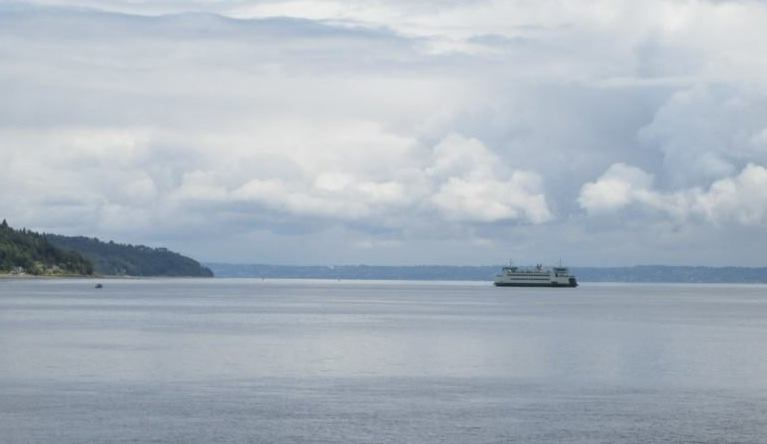
\includegraphics[scale = .55]{ferry2.jpg}
\end{center}
\end{figure}



\end{document}  